\documentclass[11pt]{article}

\usepackage[margin=1in]{geometry}
\usepackage{graphicx}
\usepackage{amsmath,amssymb,mathtools,comment,xcolor,tikz,mdframed}
\usetikzlibrary{arrows.meta,positioning,shapes.geometric,calc,fit}
\usepackage[hidelinks]{hyperref}

\DeclareMathOperator{\Tr}{Tr}

\title{NNN simulator: theory, algorithm, and implementation}
\author{}
\date{}

\begin{document}
\maketitle
\tableofcontents

\section{Theory, algorithm, and implementation}

% Companion notes to the NNN simulator (see README.md).
% Fragment: the top level is \subsection, so it can be included inside a
% section of a larger document.
%
% Requires in the preamble:
%   \usepackage{amsmath,amssymb,mathtools,comment,xcolor,tikz,mdframed}
%   \usetikzlibrary{arrows.meta,positioning,shapes.geometric,calc,fit}
%   \DeclareMathOperator{\Tr}{Tr}      % if not already defined
% Citation keys are defined in algorithm_refs.bib.

\definecolor{partcol}{RGB}{40,60,120}
\definecolor{ratecol}{RGB}{190,95,0}
\definecolor{flankcol}{RGB}{0,120,65}
\definecolor{sigcol}{RGB}{0,140,90}

% One colour per event mechanism, used in the text, the boxed procedure and
% Figure~\ref{fig:algorithm}; black marks what all three share.
\definecolor{heapcol}{RGB}{0,90,170}
\definecolor{unifcol}{RGB}{190,95,0}
\definecolor{dircol}{RGB}{0,120,65}

These notes accompany the simulator kept in this repository, and follow it from the physics down to the code. Section~\ref{sec:simulated-model} discusses the family of stochastic lattice gases being simulated, fixes the notation, and most of the parameters the simulator takes. Section~\ref{sec:monitoring} sets up the measurement protocol considered and how it affects the observer's statistical description of the system. Section~\ref{sec:largedeviations} states the current statistics we are after and carries out the calculation that turns them into an average over trajectories and measurement records. That average is what the simulation estimates: Section~\ref{sec:algorithm} writes the estimator algorithmically, as a sequence of steps, and Section~\ref{sec:implementation} describes how those steps are numerically implemented and how much they cost. Section~\ref{sec:parameters} collects every input parameter for reference.

\subsection{The lattice gas}
\label{sec:simulated-model}

We begin with a brief overview of the classical stochastic exclusion processes implemented by the simulator. The system is a chain of $L$ sites, in which particles hop between neighbouring sites subject to the exclusion principle, that forbids double occupancy. The configuration on the chain is thus a binary occupation vector $\mathbf{n} \in \{0,1\}^L$. The chain may be open, with reservoirs at either end that inject and remove particles, or periodic, with site $L$ connected to site $1$; in the latter case, the total particle number is conserved. Figure~\ref{fig:chain} illustrates the system.



\begin{figure}[htbp]
\centering
\begin{tikzpicture}[
  site/.style   = {circle, draw, minimum size=6mm, inner sep=0pt},
  full/.style   = {site, fill=partcol, text=white},
  empty/.style  = {site, fill=white},
  res/.style    = {rectangle, draw, rounded corners=2pt, minimum width=0.95cm,
                   minimum height=1.35cm, align=center, font=\small,
                   fill=black!5},
  hop/.style    = {-{Stealth[length=2mm]}, thick, ratecol},
  bath/.style   = {-{Stealth[length=2mm]}, thick},
  lab/.style    = {font=\scriptsize, inner sep=1.5pt},
  title/.style  = {font=\bfseries\small, fill=white, inner sep=3pt},
  geo/.style    = {draw=black!55, line width=1pt, rounded corners=3pt},
  box/.style    = {inner sep=3.2mm, draw=none},
]

%% ------------------------------------------------- the periodic ring
\begin{scope}
  \def\R{1.28}
  \foreach \i/\occ in {0/1,1/0,2/1,3/1,4/0,5/1,6/0,7/0,8/1,9/0} {
    \ifnum\occ=1 \node[full]  (r\i) at ({90-36*\i}:\R) {};
    \else        \node[empty] (r\i) at ({90-36*\i}:\R) {}; \fi
  }
  \draw[hop] ({90-36*2+13}:{\R+0.42}) arc[start angle={90-36*2+13},
             end angle={90-36*3-13}, radius={\R+0.42}];
  \draw[flankcol, thick, dashed] ({90-36*9}:{\R+0.36})
        arc[start angle={90-36*9}, end angle={90-36*10}, radius={\R+0.36}];
  \node[lab, flankcol] (cb) at ({90-36*9.6}:{\R+1.12}) {closing bond};
  \node[lab] at ({90-5}:{\R+0.62}) {$1$};
  \node[lab] at ({90-36*9+5}:{\R+0.64}) {$L$};
\end{scope}
\node[box, fit=(r0)(r1)(r2)(r3)(r4)(r5)(r6)(r7)(r8)(r9)(cb)] (ringbox) {};

%% ------------------------------------------------- the open chain
\begin{scope}[xshift=5.15cm, x=0.92cm]
  \foreach \i/\occ in {0/1,1/0,2/1,3/1,4/0,5/1,6/0,7/0} {
    \ifnum\occ=1 \node[full] (s\i) at (\i,0) {}; \else \node[empty] (s\i) at (\i,0) {}; \fi
  }
  \node[res, left=5mm of s0]  (resa) {$\rho_{\rm L}$};
  \node[res, right=5mm of s7] (resb) {$\rho_{\rm R}$};
  \draw[bath] (resa.east) to[bend left=32] node[lab, above] {$\alpha$} (s0.west);
  \draw[bath] (s0.west) to[bend left=32] node[lab, below] {$\gamma$} (resa.east);
  \draw[bath] (resb.west) to[bend right=32] node[lab, above] {$\delta$} (s7.east);
  \draw[bath] (s7.east) to[bend right=32] node[lab, below] {$\beta$} (resb.west);
  \draw[hop] (s3.north) to[bend left=45]
        node[lab, above] {$c_\rightarrow$} (s4.north);
  \draw[hop] (s5.south) to[bend left=45]
        node[lab, below] {$c_\leftarrow$} (s4.south);
  \draw[flankcol, thick, dashed, rounded corners=3pt]
        ($(s2.north west)+(-1.2mm,3mm)$) rectangle
        ($(s5.south east)+(1.2mm,-3mm)$);
  \node[lab, flankcol] (win) at (3.5,-1.12)
        {four-site window $(n_{b-1}, n_b, n_{b+1}, n_{b+2})$};
  \node[lab] (idxtop) at (2,1.36) {$b\!-\!1$};
  \node[lab] at (3,1.36) {$b$};
  \node[lab] at (4,1.36) {$b\!+\!1$};
  \node[lab] at (5,1.36) {$b\!+\!2$};
  \node[lab] (nsites) at (3.5,-1.72) {$L$ sites};
  \draw[|-|, gray] (-0.35,-1.48) -- (7.35,-1.48);
\end{scope}
\node[box, fit=(resa)(resb)(idxtop)(nsites)(win)] (chainbox) {};

%% ------------------------------------------------- equal-height frames
\node[fit=(ringbox)(chainbox), draw=none, inner sep=0pt] (both) {};
\draw[geo] (ringbox.west  |- both.south) rectangle (ringbox.east  |- both.north);
\draw[geo] (chainbox.west |- both.south) rectangle (chainbox.east |- both.north);
\node[title] at (ringbox.center  |- both.north) {periodic ring};
\node[title] at (chainbox.center |- both.north) {open chain};

\end{tikzpicture}
\caption{The two geometries; filled circles are occupied sites. On the right, an open chain of $L$ sites between two reservoirs: a particle hops across a bond only into an empty neighbour, at a rate set by its own two sites together with the two flanking them (dashed), while the reservoirs inject and remove at the four boundary rates. On the left, the periodic ring, where site $L$ is joined back to site $1$: the reservoirs are absent, the particle number is conserved, and every bond has both of its flanking sites.}
\label{fig:chain}
\end{figure}
Since particles can only jump left/right to adjacent sites, it is important to define a \emph{bond} as a pair of neighbouring sites $(b, b+1)$ across which a jumping event occurs. The number of bonds $\ell$ varies from $\ell=L-1$ in the open chain to $\ell=L$ on a periodic ring. A right hop moves a particle from $b$ to $b+1$ at rate $c_\rightarrow$ and requires $n_b = 1$, $n_{b+1} = 0$; a left hop is its mirror image at rate $c_\leftarrow$. On an open chain four reservoir transitions act on the ends, injecting (removing) particles at rate $\alpha$ ($\gamma$) on the left and $\delta$ ($\beta$) on the right, thus giving reservoir densities $\rho_{\rm L} = \alpha/(\alpha + \gamma)$ and $\rho_{\rm R} = \delta/(\delta + \beta)$.

We first consider an external field $E$ biasing the hopping. It distinguishes the jump rate in both directions through
\begin{equation}
    c_\rightarrow = p_0 \, w, \qquad c_\leftarrow = q_0 \, w,
    \qquad p_0 = e^{E/\ell}, \quad q_0 = e^{-E/\ell},
    \label{eq:field}
\end{equation}
where $w > 0$ is a rate that is independent of the jump direction. A positive $E$ therefore makes a particle more likely to move right than left, a negative one reverses the preference, and $E = 0$ leaves the two directions balanced. Since $p_0 q_0 = 1$, the field fixes only the ratio of the two rates and not their scale. Figure~\ref{fig:field} shows the three cases. 
\begin{figure}[htbp]
\centering
\begin{tikzpicture}[
  site/.style  = {circle, draw, minimum size=6.5mm, inner sep=0pt},
  full/.style  = {site, fill=partcol},
  empty/.style = {site, fill=white},
  lab/.style   = {font=\scriptsize, inner sep=1.5pt},
  panel/.style = {font=\small},
]
\foreach \case/\rw/\lw/\name [count=\p from 0] in {%
    0/0.5pt/1.9pt/{$E<0$}, 1/1.2pt/1.2pt/{$E=0$}, 2/1.9pt/0.5pt/{$E>0$}} {
  \begin{scope}[xshift=\p*4.3cm]
    \node[empty] (a\p) at (-0.85,0) {};
    \node[full]  (b\p) at (0,0)     {};
    \node[empty] (c\p) at (0.85,0)  {};
    \draw[-{Stealth[length=2.2mm]}, ratecol, line width=\rw]
         (b\p.north) to[bend left=42] node[lab, above] {$p_0$} (c\p.north);
    \draw[-{Stealth[length=2.2mm]}, ratecol, line width=\lw]
         (b\p.south) to[bend left=42] node[lab, below] {$q_0$} (a\p.south);
    \node[panel] at (0,-1.35) {\name};
  \end{scope}
}
\end{tikzpicture}
\caption{The external field $E$ biases the two hop directions against each
other, the thicker arrow marking the faster rate. It enters as
$p_0 = e^{E/\ell}$ to the right and $q_0 = e^{-E/\ell}$ to the left, so the
product $p_0 q_0 = 1$ is fixed and only the ratio changes with $E$. The
weight $w$ multiplying them is the same in both directions until the interaction
of equation~\ref{eq:rates} is switched on.}
\label{fig:field}
\end{figure}

In the family of models that we consider, the rate $w$ is not a single number but depends on the occupations of the two sites flanking the hopping pair, that is, on the four-site window $(n_{b-1}, n_b, n_{b+1}, n_{b+2})$. More specifically, the rates become
\begin{equation}
    c_\rightarrow = p_0 \, w_\rightarrow(n_{b-1},n_{b+2}), \qquad
    c_\leftarrow = q_0 \, w_\leftarrow(n_{b-1},n_{b+2}).
    \label{eq:rates}
\end{equation}
Letting the rate depend on the flanking pair is among the simplest ways of giving
the particles an interaction. Equation~\ref{eq:rates} is the whole family the
simulator implements: the eight weights may be handed to it directly, which is
the option it calls \texttt{NNN}. Two members of the family are common enough
to be worth naming, and are provided as options of their own:


\begin{itemize}
\item \textbf{WASEP}, the weakly asymmetric simple exclusion process: all eight weights are equal to one, so the flanking sites play no role and the particles are free apart from the exclusion itself. Its open-boundary steady state is known exactly from the matrix ansatz \cite{derrida1993exact}, and its current large deviations are the setting in which the additivity principle was formulated \cite{bodineau2004current}. It is therefore the case against which the simulator can be checked.
\item \textbf{KLS}, the Katz--Lebowitz--Spohn model \cite{katz1984nonequilibrium}: the weights are built from two parameters,
\begin{equation}
    w_\rightarrow(a,d) = 1 + \delta_{\text{KLS}}(1 - a - d) + \epsilon (a - d), \qquad w_\leftarrow(a,d) = w_\rightarrow(d,a),
\end{equation}
a left hop being the spatial inversion of a right one. $\epsilon$ and $\delta_{\rm KLS}$ must satisfy $|\epsilon| < 1$ and $|\delta_{\text{KLS}}| < 1$ for every rate to stay positive. A positive $\epsilon$ makes the particles repel one another, while $\delta_{\text{KLS}}$ breaks the symmetry between particles and holes. Setting both to zero returns the WASEP weights.
\begin{figure}[htbp]
\centering
\begin{tikzpicture}[
  x=0.72cm,
  site/.style  = {circle, draw, minimum size=5mm, inner sep=0pt},
  full/.style  = {site, fill=partcol},
  empty/.style = {site, fill=white},
  hop/.style   = {-{Stealth[length=1.6mm]}, thick, ratecol},
]
\foreach \panel/\a/\d/\rate [count=\p from 0] in {%
   0/0/0/{1+\delta_{\text{KLS}}}, 1/0/1/{1-\epsilon},
   2/1/0/{1+\epsilon}, 3/1/1/{1-\delta_{\text{KLS}}}} {
  \begin{scope}[xshift=\p*3.15cm]
    \ifnum\a=1 \node[full] (a\p) at (0,0) {}; \else \node[empty] (a\p) at (0,0) {}; \fi
    \node[full]  (b\p) at (1,0) {};
    \node[empty] (c\p) at (2,0) {};
    \ifnum\d=1 \node[full] (d\p) at (3,0) {}; \else \node[empty] (d\p) at (3,0) {}; \fi
    \draw[hop] (b\p.north) to[bend left=45] (c\p.north);
    \node[font=\scriptsize] at (1.5,-0.85) {$(a,d)=(\a,\d)$};
    \node[font=\scriptsize, ratecol] at (1.5,-1.35) {$w_\rightarrow = \rate$};
  \end{scope}
}
\end{tikzpicture}
\caption{The four rate groups of a right hop; the hopping pair is the middle one, and the two outer circles are the flanking sites. The same hop across the same bond proceeds at four different rates depending only on the occupations of the two sites beside it; the rates shown are those of the Katz--Lebowitz--Spohn model. Left hops are the mirror image, $w_\leftarrow(a,d) = w_\rightarrow(d,a)$. Setting $\epsilon = \delta_{\text{KLS}} = 0$ makes all four equal and recovers WASEP.}
\label{fig:classes}
\end{figure}
\end{itemize}

We stress that none of these interaction rates involves the external field, which multiplies them as described above in Eq.~(\ref{eq:rates}).


\subsection{Monitoring: the system as an observer sees it}
\label{sec:monitoring}

The lattice gas of Section~\ref{sec:simulated-model} is now placed under continuous observation. A measurement device is coupled to every site and reports on its occupation through an output signal $\mathcal{S}$, which is what the observer actually sees; Figure~\ref{fig:measurement} sketches the arrangement. How faithfully that signal tracks the true occupation is set by a single parameter $k$, the measurement strength. For a perfect measurement device that is memoryless, the probability of a given signal, conditioned on a configuration trajectory $\mathcal{C}$, is
\begin{equation}\label{eq:S|C}
    \mathbb{P}_{\left[0,t\right]}\left(\mathcal{S}|\mathcal{C}\right) \propto \exp\left[-\frac{k}{2L^2}\int_0^t dt' \sum_{i=1}^L \left(\mathcal{S}_i(t') -\mathcal{C}_i(t')\right)^2\right],
\end{equation}
where $\mathcal{S}_i(t')\in \mathbb{R}$ is the signal at site $i$ and $\mathcal{C}_i(t') \coloneqq 2 n_i(t)-1 \in\{-1,1\}$ is the configuration written in the $\pm 1$ convention. Bayes' rule then inverts this into the observer's statistical description of the system given the recorded signal,
\begin{equation}\label{eq:C|S}
    \mathbb{P}_{\left[0,t\right]}\left(\mathcal{C}|\mathcal{S}\right) \propto \mathbb{P}_{\left[0,t\right]}\left(\mathcal{C}\right)\,\exp\left[-\frac{k}{2L^2}\int_0^t dt' \sum_{i=1}^L \left(\mathcal{S}_i(t') -\mathcal{C}_i(t')\right)^2\right] .
\end{equation}

\begin{figure}[htbp]
\centering
\begin{tikzpicture}[
  site/.style   = {circle, draw, minimum size=4.5mm, inner sep=0pt},
  full/.style   = {site, fill=partcol},
  empty/.style  = {site, fill=white},
  anc/.style    = {rectangle, draw, minimum size=3.4mm, inner sep=0pt,
                   fill=black!8, font=\tiny},
  tap/.style    = {-{Stealth[length=1.4mm]}, gray},
  big/.style    = {-{Stealth[length=2.4mm]}, very thick},
  lab/.style    = {font=\scriptsize, inner sep=2pt},
  ttl/.style    = {font=\scriptsize\bfseries},
]
%% the system
\begin{scope}
  \foreach \i/\occ in {0/1,1/0,2/1,3/1,4/0,5/1} {
    \ifnum\occ=1 \node[full] (p\i) at (\i*0.6,0) {};
    \else        \node[empty] (p\i) at (\i*0.6,0) {}; \fi
    \node[anc] (q\i) at (\i*0.6,-0.95) {};
    \draw[tap] (p\i) -- (q\i);
  }
  \node[ttl] at (1.5,0.75) {the system};
  \node[lab] at (1.5,-1.5) {ancillas, read out every $\Delta t$};
\end{scope}
%% the record
\begin{scope}[xshift=7.1cm, yshift=-0.45cm]
  \node[rectangle, draw, rounded corners=2.5pt, minimum width=4.3cm,
        minimum height=2.7cm, fill=black!6] (case) at (0,0) {};
  \node[rectangle, draw, fill=black!88, minimum width=3.5cm,
        minimum height=1.7cm] (screen) at (0,0.32) {};
  \foreach \gx in {-1.5,-1.0,...,1.5}
      \draw[white!22, very thin] (\gx,-0.53) -- (\gx,1.17);
  \foreach \gy in {-0.4,0,...,1.1}
      \draw[white!22, very thin] (-1.75,\gy) -- (1.75,\gy);
  \draw[sigcol, thick]
     plot coordinates {(-1.72,0.35) (-1.58,0.62) (-1.44,0.28) (-1.30,0.55)
       (-1.16,0.14) (-1.02,0.48) (-0.88,0.72) (-0.74,0.31) (-0.60,0.08)
       (-0.46,0.44) (-0.32,0.66) (-0.18,0.22) (-0.04,0.51) (0.10,0.83)
       (0.24,0.38) (0.38,0.12) (0.52,0.47) (0.66,0.69) (0.80,0.26)
       (0.94,0.58) (1.08,0.33) (1.22,0.05) (1.36,0.42) (1.50,0.64)
       (1.64,0.29) (1.72,0.46)};
  \node[font=\tiny, white] at (-1.12,1.00) {$S_j(t)$};
  \foreach \kx in {-1.2,-0.4,0.4,1.2}
      \node[circle, draw, minimum size=3.2mm, inner sep=0pt, fill=white]
            at (\kx,-1.02) {};
  \node[ttl] at (0,1.72) {the record};
\end{scope}
%% the observer
\begin{scope}[xshift=11.3cm, yshift=-0.55cm]
  \node[circle, draw, minimum size=6mm, inner sep=0pt] (head) at (0,0.35) {};
  \draw[thick] (0,0.05) -- (0,-0.6);
  \draw[thick] (0,-0.12) -- (-0.32,-0.42);
  \draw[thick] (0,-0.12) -- (0.32,-0.42);
  \draw[thick] (0,-0.6) -- (-0.26,-1.05);
  \draw[thick] (0,-0.6) -- (0.26,-1.05);
  \node[ellipse, draw, minimum width=2.7cm, minimum height=1.7cm,
        fill=black!3] (bub) at (1.35,1.5) {};
  \node[circle, draw, minimum size=2.4mm, fill=black!3] at (0.52,0.72) {};
  \node[circle, draw, minimum size=1.4mm, fill=black!3] at (0.34,0.55) {};
  \begin{scope}[shift={(1.35,1.38)}, x=0.175cm, y=0.5cm]
    \foreach \bx/\bh in {-3/0.30,-2/0.52,-1/0.68,0/0.62,1/0.44,2/0.26,3/0.13}
        \draw[partcol, line width=1.5pt] (\bx,0) -- (\bx,\bh);
    \draw[gray, thin] (-3.6,0) -- (3.6,0);
  \end{scope}
  \node[font=\tiny] at (1.35,2.05) {$\mathcal{P}(\vec{X}\,|\,\vec{a})$};
  \node[ttl] at (0.55,-1.5) {the observer};
\end{scope}
\draw[big] (3.55,-0.5) -- node[lab, above] {$\vec{a}$} (4.85,-0.5);
\draw[big] (9.45,-0.5) -- node[lab, above] {Bayes} (10.55,-0.5);
\end{tikzpicture}
\caption{The monitoring, schematically. An ancilla is coupled to every site and read out every $\Delta t$, so what leaves the system is not its configuration but a noisy record $\vec{a}$ of it. The observer never sees the chain; they see the record, and from it maintain a probability distribution over configurations, updated by Bayes' rule as each outcome arrives. The population of walkers the simulator evolves is a Monte Carlo representation of exactly that distribution.}
\label{fig:measurement}
\end{figure}

Algorithmically this calls for two objects rather than one. The first is a "physical" realisation of the stochastic process, the trajectory that is actually taking place, on which the measurements are performed according to Eq.~(\ref{eq:S|C}). The second is the observer's description of it, which the simulator represents by a population of walkers, each weighted by its likelihood under Eq.~(\ref{eq:C|S}) as further outcomes arrive. Denoting the physical trajectory by $\mathcal{C}^{(0)}$, the signal follows the law
\begin{equation}\label{eq:SWiener}
    \mathcal{S}_i(t') =\mathcal{C}^{(0)}_i(t') + \frac{L^2}{k}\,\frac{dW_i(t')}{dt},
\end{equation}
where $dW_i(t')$ is a Wiener process with $\overline{dW_i^2}=\frac{k}{L^2}\,dt$. Using this result in Eq.~(\ref{eq:C|S}) gives 
\begin{equation}\label{eq:C|C0W}
    \mathbb{P}_{\left[0,t\right]}\left(\mathcal{C}\,\left|\mathcal{S}\right.\right) \propto \mathbb{P}_{\left[0,t\right]}\left(\mathcal{C}\right)\,\exp\left[\frac{k}{L^2}\int_0^t dt' \sum_{i=1}^L \mathcal{C}_i(t')\, \mathcal{C}^{(0)}_i(t')+\sum_{i=1}^L\int_0^t dW_i(t') \mathcal{C}_i(t') \right] .
\end{equation}

\subsection{Large deviations}
\label{sec:largedeviations}

Having specified the dynamics and the measurement protocol, we can now turn to the observable whose fluctuations the simulator is designed to resolve: the particle current. Recall that $\ell$ is the number of bonds, with $\ell=L-1$ for an open chain and $\ell=L$ for a periodic ring. For each bond $b$, let $Q_b(t)$ denote the net number of particles that have crossed it by time $t$, counting rightward and leftward passages as $+1$ and $-1$, respectively, and let $J_b(t)=Q_b(t)/t$ be the corresponding time-averaged current. Particle conservation bounds $Q_b(t)-Q_{b'}(t)$ by the change in particle number in the segment between the two bonds. This difference cannot grow with time, and therefore $J_b(t)-J_{b'}(t)\to0$ as $t\to\infty$. We may thus average over bonds without changing the long-time current:
\begin{equation}
    J(t) := \frac{1}{\ell}\sum_{b=1}^{\ell} J_b(t)
    = \frac{1}{t\,\ell}\sum_{b=1}^{\ell} Q_b(t)
    =:\frac{\mathcal{Q}_t[\mathcal{C}]}{t}.
\end{equation}

Although the bond dependence disappears from the long-time current, $J(t)$ remains a random variable that differs between realisations of the dynamics. Its distribution concentrates around the mean at long times, while an atypical value $j$ is exponentially suppressed:
$\mathbb{P}\left(J(t) \simeq j\right) \asymp e^{-t\,I(j)}$, with $I$ the rate
function. All of that distribution, its rare values included, is carried by the scaled cumulant generating function
\begin{equation}
    \chi(s) = \lim_{t \to \infty} \frac{1}{t}
    \log \left\langle e^{\,s\,t\,J(t)} \right\rangle,
    \label{eq:cgf-definition}
\end{equation}
where $\left\langle \cdot \right\rangle$ denotes an average over process trajectories. Indeed, it is well-known from large-deviation theory~\cite{touchette2009large} that $\chi$ is the Legendre transform of $I$. Its derivatives at $s = 0$ give the current cumulants: the mean at first order and the variance at second order. A nonzero $s$ probes the tails of the distribution: positive values favour trajectories with an atypically large current, whereas negative values favour those with an atypically small current.

To evaluate this average, we write the integrated bond-averaged current as the trajectory functional
\begin{equation}
    \mathcal{Q}_t[\mathcal{C}] = \sum_{m=1}^{M_t}
        q\!\left(\mathcal{C}^{(m-1)} \to \mathcal{C}^{(m)}\right),
    \label{eq:counting}
\end{equation}
Here $M_t$ is the total number of transitions by time $t$, and
$\mathcal{C}^{(m)}$ is the configuration immediately after the $m$th transition. Each bulk hop contributes $+1/\ell$ to $\mathcal{Q}_t$ if it is to the right and $-1/\ell$ if it is to the left; by choice, reservoir transitions are not counted in the open case.
We shall now rewrite this average in a form suitable for simulation. For a Markov jump process, the probability of a trajectory factorises into contributions from its jumps and the waiting times between them:
\begin{equation}
    \mathbb{P}_{\left[0,t\right]}\left(\mathcal{C}\right) = \prod_{m=1}^{M_t}
        W\!\left(\mathcal{C}^{(m-1)} \to \mathcal{C}^{(m)}\right)\,
    \exp\left[-\int_0^t dt'\, R\!\left(\mathcal{C}(t')\right)\right],
    \qquad
    R(\mathcal{C}) = \sum_{\mathcal{C}'} W\!\left(\mathcal{C} \to \mathcal{C}'\right),
\end{equation}
Here $R(\mathcal{C})$ is the escape rate from the configuration $\mathcal{C}$. Multiplication by $e^{s\mathcal{Q}_t[\mathcal{C}]}$ attaches a factor $e^{s q(\mathcal{C} \to \mathcal{C}')}$ to each bulk transition. We absorb these factors into the \emph{tilted} rates,
\begin{equation}
    W_s\!\left(\mathcal{C} \to \mathcal{C}'\right) =
    W\!\left(\mathcal{C} \to \mathcal{C}'\right)\,
    e^{\,s\,q(\mathcal{C} \to \mathcal{C}')}.
    \label{eq:tilted-rates}
\end{equation}
For the bulk rates, where $q=\pm1/\ell$, this factor is equivalent to replacing the field $E$ by $E+s$. Equation~\ref{eq:rates} therefore becomes $w_\rightarrow(a,d)\,p_s$ and $w_\leftarrow(a,d)\,q_s$, with $p_s=e^{(E+s)/\ell}$ and $q_s=e^{-(E+s)/\ell}$. The reservoir rates remain unchanged because, by choice, reservoir transitions do not contribute to the current and hence have $q=0$.
The tilted rates define a new escape rate $R_s(\mathcal{C}) = \sum_{\mathcal{C}'} W_s(\mathcal{C} \to \mathcal{C}')$. Because the waiting-time factor in $\mathbb{P}_{\left[0,t\right]}\left(\mathcal{C}\right)$ still contains the original escape rate $R$, changing the jump rates from $W$ to $W_s$ leaves a correction along the trajectory that we call the counting-field potential,
\[
    V_s(\mathcal{C}):=R_s(\mathcal{C})-R(\mathcal{C}).
\]
The change of trajectory measure is then
\begin{equation}
    \mathbb{P}_{\left[0,t\right]}\left(\mathcal{C}\right)\, e^{s\mathcal{Q}_t[\mathcal{C}]}
    = \mathbb{P}^{(s)}_{\left[0,t\right]}\left(\mathcal{C}\right) \,
      \exp\left[\int_0^t dt'\,
        V_s\!\left(\mathcal{C}(t')\right)\right],
    \label{eq:tilt-split}
\end{equation}
Here $\mathbb{P}^{(s)}_{\left[0,t\right]}$ is the trajectory probability of the Markov process generated by $W_s$. Equation~\ref{eq:tilt-split} therefore separates the bias into two parts: the modified dynamics and the escape-rate correction accumulated along each trajectory. Averaging this identity and taking the long-time limit gives the unmonitored CGF,
\begin{equation}
    \chi_0(s) = \lim_{t \to \infty} \frac{1}{t} \log \left\langle
    \exp\left[\int_0^t dt'\,
    V_s\!\left(\mathcal{C}(t')\right)\right]
    \right\rangle_{\!s},
    \label{eq:cgf-tilted}
\end{equation}
where $\langle\cdot\rangle_s$ denotes an average over those tilted dynamics.

To include measurements, we use equation~\ref{eq:C|C0W} directly. The physical trajectory $\mathcal{C}^{(0)}$ and the Wiener process $W$ together specify the measurement record, and they assign each candidate trajectory $\mathcal{C}$ the additional weight $e^{\mathcal{M}_{\mathcal{C}^{(0)},W}[\mathcal{C}]}$, where
\[
    \mathcal{M}_{\mathcal{C}^{(0)},W}[\mathcal{C}]
    := \frac{k}{L^2}\int_0^t dt'\sum_{i=1}^L
    \mathcal{C}_i(t')\mathcal{C}^{(0)}_i(t')
    +\sum_{i=1}^L\int_0^t \mathcal{C}_i(t')\,dW_i(t').
\]
Combining this measurement weight with the change of measure in equation~\ref{eq:tilt-split}, and normalising by the corresponding untilted conditional weight, gives the monitored CGF directly as
\begin{equation}
\begin{split}
    \chi_k(s) = \lim_{t\to\infty}\frac{1}{t}\,
    \mathbb{E}_{\mathcal{C}^{(0)},W}\!\left[
    \log
    \frac{
    \left\langle \exp\!\left[
        \displaystyle\int_0^t dt'\,
        V_s(\mathcal{C}(t'))
        +\mathcal{M}_{\mathcal{C}^{(0)},W}[\mathcal{C}]
    \right]\right\rangle_s
    }{
    \left\langle
        e^{\mathcal{M}_{\mathcal{C}^{(0)},W}[\mathcal{C}]}
    \right\rangle_0
    }
    \right].
\end{split}
    \label{eq:cgf-monitored}
\end{equation}
Here the outer expectation averages over the physical trajectory $\mathcal{C}^{(0)}$ and the Wiener process $W$ with the laws specified in Section~\ref{sec:monitoring}; the denominator inside the logarithm is averaged over the original, untilted dynamics. The It\^o integral in $\mathcal{M}_{\mathcal{C}^{(0)},W}$ typically grows as $\sqrt{t}$, whereas the other terms in the exponent grow linearly with $t$. Its contribution to the logarithm is therefore sublinear and disappears after division by $t$ in the long-time limit.
As a consequence, removing the It\^o term from both the numerator and its normalisation leaves the measurement potential
\[
    U_k(\mathcal{C},t)
    :=\frac{k}{L^2}\sum_{i=1}^L
    \mathcal{C}_i\mathcal{C}^{(0)}_i(t).
\]
Together with the counting-field potential, it defines the total potential
\[
    \Phi_{s,k}(\mathcal{C},t)
    :=V_s(\mathcal{C})+U_k(\mathcal{C},t).
\]
The monitored CGF can then be written as
\begin{equation}
\begin{split}
    \chi_k(s)
    ={}& \lim_{t\to\infty}\frac{1}{t}\,
    \mathbb{E}_{\mathcal{C}^{(0)}}\!\left[
    \log
    \frac{
    \left\langle\exp\left[\int_0^t dt'\,
        \Phi_{s,k}\!\left(\mathcal{C}(t'),t'\right)
    \right]\right\rangle_s
    }{
    \left\langle\exp\left[\int_0^t dt'\,
        \Phi_{0,k}\!\left(\mathcal{C}(t'),t'\right)
    \right]\right\rangle_0
    }
    \right],
\end{split}
    \label{eq:cgf-simulated-1}
\end{equation}
Here $\Phi_{0,k}=U_k$ because $V_0=0$. The numerator and denominator correspond to two evolutions that we can simulate, at $s$ and $s=0$, respectively. When $k=0$, the measurement potential and its normalisation vanish, recovering equation~\ref{eq:cgf-tilted}.

Rather than waiting until the end of a trajectory to evaluate the averages in equation~\ref{eq:cgf-simulated-1}, we can update the trajectory weights as the dynamics proceeds. For a fixed physical trajectory $\mathcal{C}^{(0)}$, let $\widetilde{P}_s(\mathcal{C},t\mid\mathcal{C}^{(0)})$ be the total weight of all tilted trajectories that end in configuration $\mathcal{C}$ at time $t$:
\begin{equation}
    \widetilde{P}_s(\mathcal{C},t\mid\mathcal{C}^{(0)})
    :={}\left\langle
    \mathbf{1}_{\{\mathcal{C}'(t)=\mathcal{C}\}}
    \exp\!\left[\int_0^t d\tau\,
      \Phi_{s,k}(\mathcal{C}'(\tau),\tau)\right]
    \right\rangle_s,\,
    Z_s(t\mid\mathcal{C}^{(0)}):={}\sum_{\mathcal{C}}
      \widetilde{P}_s(\mathcal{C},t\mid\mathcal{C}^{(0)}).
\end{equation}
Here $\mathcal{C}'$ is the trajectory being averaged over. Summing over the final configuration removes the endpoint condition, so $Z_s$ is precisely the numerator of equation~\ref{eq:cgf-simulated-1}; at $s=0$, the same expression gives its denominator. Since $\widetilde{P}_s$ does not generally sum to one, we divide it by $Z_s$ to obtain the probability distribution
\[
    P_s(\mathcal{C},t\mid\mathcal{C}^{(0)})
    :=\frac{\widetilde{P}_s(\mathcal{C},t\mid\mathcal{C}^{(0)})}
    {Z_s(t\mid\mathcal{C}^{(0)})}.
\]
Thus $\sum_{\mathcal{C}}P_s(\mathcal{C},t\mid\mathcal{C}^{(0)})=1$ for every $s$. For a generic observable $A$, write the average
\[
    \langle A \rangle_s(t)
    :=\sum_{\mathcal{C}}A(\mathcal{C},t)
      P_s(\mathcal{C},t\mid\mathcal{C}^{(0)}).
\]
The probabilities $P_s(\mathcal{C},t\mid\mathcal{C}^{(0)})$ evolve according to
\begin{equation}
\begin{split}
    \partial_t P_s(\mathcal{C},t\mid\mathcal{C}^{(0)})
    ={}& \sum_{\mathcal{C}'\neq\mathcal{C}}
    W_s(\mathcal{C}'\to\mathcal{C})
    P_s(\mathcal{C}',t\mid\mathcal{C}^{(0)})
    -R_s(\mathcal{C})
    P_s(\mathcal{C},t\mid\mathcal{C}^{(0)}) \\
    &+\bigl[\Phi_{s,k}(\mathcal{C},t)
    -\langle \Phi_{s,k}\rangle_s(t)\bigr]
    P_s(\mathcal{C},t\mid\mathcal{C}^{(0)}),
\end{split}
    \label{eq:tilted-probability-evolution}
\end{equation}
where the chosen initial distribution fixes $P_s(\mathcal{C},0\mid\mathcal{C}^{(0)})=P_{\mathrm{ini}}(\mathcal{C})$. The first line describes the usual probability flow generated by the tilted rates $W_s$, while the second redistributes probability towards configurations with a larger $\Phi_{s,k}$. Subtracting the average of $\Phi_{s,k}$ ensures that the probabilities continue to sum to one, and the corresponding overall factor is recorded in $Z_s$:
\[
    \frac{d}{dt}\log Z_s(t\mid\mathcal{C}^{(0)})
    =\langle\Phi_{s,k}\rangle_s(t),
    \qquad
    Z_s(t\mid\mathcal{C}^{(0)})
    =\exp\!\left[\int_0^t dt'\,
      \langle\Phi_{s,k}\rangle_s(t')\right].
\]
Using $Z_s$ for the numerator and $Z_0$ for the denominator, equation~\ref{eq:cgf-simulated-1} becomes
\begin{equation}
\begin{split}
    \chi_k(s)
    ={}&\lim_{t\to\infty}\frac{1}{t}
    \mathbb{E}_{\mathcal{C}^{(0)}}\!\left[
      \log Z_s(t\mid\mathcal{C}^{(0)})
      -\log Z_0(t\mid\mathcal{C}^{(0)})\right]\\
    ={}&\lim_{t\to\infty}\frac{1}{t}
    \mathbb{E}_{\mathcal{C}^{(0)}}\!\left[
      \int_0^t dt'\,
      \bigl(\langle\Phi_{s,k}\rangle_s(t')
      -\langle\Phi_{0,k}\rangle_0(t')\bigr)\right].
\end{split}
\label{eq:cgf-simulated-2}
\end{equation}
The two equalities in equation~\ref{eq:cgf-simulated-2} lead to independent numerical estimates of the same growth rate: one from $\log Z_s/t$ and the other from the time average of $\langle\Phi_{s,k}\rangle_s$. Their agreement provides a useful cross-check. The monitored CGF is obtained only after subtracting the corresponding result at $s=0$.

Finally, there exists a third route to the CGF that uses its derivative. Differentiating its defining logarithm, Eq.~(\ref{eq:cgf-definition}), with respect to $s$ brings down the integrated current $\mathcal{Q}_t$. Therefore
\begin{equation}
    \chi_k'(s)
    =\lim_{t\to\infty}\frac{1}{t}\,
      \mathbb{E}_{\mathcal{C}^{(0)}}\!\left[
      \bigl\langle\mathcal{Q}_t\bigr\rangle_{s}\right],
    \qquad
    \chi_k(s)=\int_0^s ds'\,\chi_k'(s').
    \label{eq:cgf-derivative}
\end{equation}
The second identity follows from $\chi_k(0)=0$, so averaging $\mathcal{Q}_t/t$ at several values of $s$ and integrating over $s$ gives a third estimate of the CGF.

\subsection{The algorithm}
\label{sec:algorithm}

The algorithm represents the weighted trajectory ensemble by a population of $M$ copies of the system, called \emph{walkers}. Each walker evolves exactly in continuous time under the tilted rates $W_s$ of equation~\ref{eq:tilted-rates}, using the Gillespie algorithm \cite{gillespie1976general,gillespie1977exact}, and carries the weight $\omega_i$ generated by the total potential $\Phi_{s,k}$; the letter $\omega$ is kept for this weight alone, the rate weights $w_\rightarrow, w_\leftarrow$ of equation~\ref{eq:rates} being a different object. If these weights were allowed to evolve freely, their ratios would grow exponentially with time and the average would soon be dominated by a few walkers. The cloning method \cite{giardina2006direct,lecomte2007numerical} controls this growth by introducing cloning times at which the walkers are resampled in proportion to their weights: walkers with large weights are replicated, whereas those with small weights are removed. Resampling keeps the weight spread manageable and directs the population towards the trajectories that contribute more to the weighted distribution. When the cloning times are placed is a matter of efficiency rather than correctness, and how they are found depends on the specific algorithm implementation, so both are settled in the notes below the boxed procedure, once the three implementations we consider are in place.

Written as a sequence of steps, with $M$ the population size and $t_{\max}$ the final time, the algorithm is as follows:

\begin{mdframed}[
    linewidth=0.8pt,
    roundcorner=3pt,
    backgroundcolor=black!5,
    innerleftmargin=8pt,
    innerrightmargin=8pt,
    innertopmargin=8pt,
    innerbottommargin=8pt]
\begin{enumerate}
\item \textbf{Initialise.} Build $M$ walkers in the requested initial configuration, each with weight one, and one reference trajectory (for $k = 0$ the reference trajectory is irrelevant and can be omitted). Set $t = 0$ and the accumulated normalisation $\log Z_s = 0$.

\item \textbf{Choose the next stop.}$^{\ddagger}$ A \emph{stop} is an instant at which the whole population is brought to a common time and may be examined. It is the earliest of the following possibilities: the next scheduled resampling instant, the next recording time, and $t_{\max}$.

\item \textbf{Evolve to the stop.}$^{\dagger}$ Walker events must be generated with the tilted rates $W_s$ until the whole population reaches the stop. When a reference trajectory exists, it must be evolved alongside the walkers until the stop, but with the unbiased rates $W_0$. We consider three distinct implementations of this step.

\smallskip
\noindent\textcolor{heapcol}{\textbf{Heap.}} Every process --- each walker, and the reference when monitoring is on --- holds one pending event time, drawn from its own escape rate $R_s(\mathcal{C})$. The mechanism is named after where those $M+1$ times are kept: a binary heap, which holds the earliest of them at its root. Then, repeat the following instructions while the earliest pending time lies before the stop:
\begin{enumerate}
\item Read the root of the heap and advance the global clock to that time.
\item Select one possible transition of that walker with probability proportional to its tilted rate, apply it, and update the integrated current by the increment $q(\mathcal{C}\to\mathcal{C}')$.
\item Update the list of allowed transitions locally, around the bond that changed.
\item Recompute that process's tilted escape rate $R_s(\mathcal{C})$, the sum of the rates of all transitions now allowed to it, draw its new pending time $t + \text{Exponential}(R_s(\mathcal{C}))$, and sift that one entry back into place in the heap. Every other process keeps the pending event time it already had.
\end{enumerate}
When the earliest pending time falls beyond the stop, advance the global clock to the stop and finish. The whole population is thus at one time at every instant.

Note the advantages of the heap in this implementation: accessing the earliest pending time is $O(1)$, and updating the heap with a new entry takes $O(\log M)$. A flat list would instead have to be scanned in full, at a cost of $O(M)$ per event, to find the same minimum.

\smallskip
\noindent\textcolor{dircol}{\textbf{Direct.}} The same events as in \textcolor{heapcol}{\textbf{Heap}}, but generated one walker at a time instead of in global order. Under monitoring the reference is evolved first, alone, from the current time to the stop, and its events are stored. Then take the walkers one by one, each carrying its own pending time; for one walker, repeat while that time lies before the stop:
\begin{enumerate}
\item Advance this walker's clock to its pending event time.
\item Select one transition with probability proportional to its tilted rate, apply it, and update the integrated current by the increment $q(\mathcal{C}\to\mathcal{C}')$.
\item Update the list of allowed transitions locally, around the bond that changed.
\item Recompute this walker's tilted escape rate $R_s(\mathcal{C})$ and draw its new pending time $t + \text{Exponential}(R_s(\mathcal{C}))$.
\end{enumerate}
When the pending time falls beyond the stop, advance this walker's clock to the stop and pass to the next walker. A walker is therefore carried all the way to the stop before the next one starts, and no two walkers share a time until they all reach it.

\smallskip
\noindent\textcolor{unifcol}{\textbf{Uniformized.}} One clock for the whole population, ticking faster than any configuration can demand, with the excess removed by rejection. With $w_{\max}$ the heaviest of the eight rates of equation~\ref{eq:rates} and $N_b$ the number of bonds, the proposal rate of one walker and of the population are, respectively,
\begin{equation}
    R_{\text{prop}} = (p_s + q_s)\, w_{\max} N_b
      + \alpha + \gamma + \delta + \beta,
    \qquad
    R_{\max} = M R_{\text{prop}},
    \label{eq:uniformized-rate}
\end{equation}
where the reservoir term is present for an open chain only. When monitoring is on, the reference adds one further process to the same clock, at a rate of the same form (but with $s=0$). The pending time belongs to the population as a whole; repeat while it lies before the stop:
\begin{enumerate}
\item Advance the global clock to the pending time.
\item Pick one process uniformly among the $M$ walkers, or the reference, in proportion to its share of $R_{\max}$; then, within it, one bond and one direction with probability proportional to $p_s$ and $q_s$, or one of the four reservoir moves in proportion to its rate.
\item Put the proposal through two tests. The first is exclusion: the hop must start from an occupied site and end on an empty one, and a reservoir move must find the boundary site in the state it needs. The second is the rate: the proposal was made at the heaviest rate $w_{\max}$, while the bond it picked can actually have some other rate $w$, so it is kept with probability $w/w_{\max}$ and dropped otherwise. A proposal that fails either test is discarded, and nothing changes. One that passes both is applied, updating the integrated current by $q(\mathcal{C}\to\mathcal{C}')$ and the list of allowed transitions locally.
\item Draw the new pending time $t + \text{Exponential}(R_{\max})$, which depends on no configuration and therefore never has to be recomputed.
\end{enumerate}
When the pending time falls beyond the stop, advance the global clock to the stop and finish. The rejections are exactly what turns the flat maximal rate back into the correct rate: a transition of weight $w$ is proposed at rate $w_{\max}$ and survives with probability $w/w_{\max}$, so ultimately it occurs at the right rate $w$.

\item \textbf{Accumulate the weights.} Over the same interval, update the weight of each walker independently according to
\begin{equation}
    \frac{d}{dt}\log \omega_i(t)
    =\Phi_{s,k}(\mathcal{C}^{(i)}(t),t).
\label{eq:walker-weight}
\end{equation}
The single numerical weight therefore contains both the counting-field and measurement contributions. Note that this is why the \textcolor{dircol}{\textbf{Direct}} construction has to evolve the reference before all the walkers: the measurement contribution compares a walker with the reference at the walker's own time, so the reference events of the whole interval must already be known when each walker is carried across it.

\item \textbf{Resample.}$^{\ddagger}$ At a resampling stop, replace the weighted population by $M$ equally weighted children, selecting their parents in proportion to the current weights. Before doing so, two matters need to be addressed. First, one may retain a diagnostic to reveal whether the weights have concentrated among too few walkers. A common choice is the effective sample size$^{\circ}$ \cite{kong1994sequential}:
\begin{equation}
    \text{ESS}=\frac{\left(\sum_i \omega_i\right)^2}{\sum_i \omega_i^2}.
    \label{eq:ess}
\end{equation}

Second, update the running estimate of the normalisation. The population mean of the weights at cloning time $t_r$ is the factor by which $Z_s$ has grown since the previous resampling, so
\begin{equation}
\log Z_s \;\mathrel{+}=\;
\log\!\left(\frac{1}{M}\sum_i \omega_i\right).
\end{equation}
Only estimators that depend on the walker weights need to be evaluated at this step, before the weights are discarded. Weight-independent estimators, such as those associated with the second equality in equation~\ref{eq:cgf-simulated-2} and with equation~\ref{eq:cgf-derivative}, can instead be evaluated at recording times, as described in the next step.

To perform a systematic resampling of the walker population \cite{kitagawa1996monte, douc2005comparison}, lay the parent weights end to end as intervals of lengths $\omega_i$ on a segment of total length $\Omega=\sum_i\omega_i$, draw one uniform offset $u$, and place $M$ equally spaced marks on the segment:
\begin{equation}
    u\sim\text{Uniform}\left(0,\Omega/M\right],
    \qquad
    u_m = u + (m-1)\,\frac{\Omega}{M},
    \qquad m = 1,\dots,M,
    \label{eq:systematic}
\end{equation}
Each mark selects the parent whose interval contains it and produces one identical child. Since interval $i$ occupies a fraction $\omega_i/\Omega$ of the segment, parent $i$ receives either $\lfloor M\omega_i/\Omega\rfloor$ or $\lceil M\omega_i/\Omega\rceil$ children, with an average of exactly $M\omega_i/\Omega$. A parent whose weight exceeds the mark spacing $\Omega/M$ cannot be lost; a lighter parent survives with probability proportional to its weight. Since one random offset determines the entire population, this procedure is cheaper and less noisy than drawing $M$ parents independently. Each child inherits its parent's complete state, including associated attributes such as the total transferred charge $\mathcal{Q}_t$, after which its weight is reset to one.

\item \textbf{Record.} If the stop is a recording time, first carry out the resampling procedure of step 5, irrespective of whether the usual resampling criterion is met. This absorbs the accumulated weights into $\log Z_s$ and replaces the weighted population by an equally weighted one. The observables below can then be recorded as unweighted population averages.

Our ultimate quantity of interest is the current CGF $\chi_k(s)$. Section~\ref{sec:largedeviations} established three distinct estimators for it: two based on the growth rate of $Z_s$, given by the two equalities in equation~\ref{eq:cgf-simulated-2}, and a third based on the mean current, given by equation~\ref{eq:cgf-derivative}. We therefore record the quantities required by each estimator.

As discussed in step 5, the first estimator is obtained from the normalisation increments accumulated at each resampling. At a recording time, write out the current value of $\log Z_s$, which gives the finite-time growth-rate estimator
\begin{equation}
    \widehat{g}^{\,(Z)}_k(s,t)
    =\frac{1}{t}\sum_{t_r\leq t}
      \log\!\left[\frac{1}{M}\sum_i \omega_i(t_r^-)\right]
    =\frac{\log Z_s(t)}{t}.
    \label{eq:cgf-estimator-normalisation}
\end{equation}
The second estimator$^{*}$ requires the instantaneous population average of the total potential, so record
\begin{equation}\label{eq:instantaneous-potential}
    \overline{\Phi}_{s,k}(t)
    :=\frac{1}{M}\sum_{i=1}^M
      \Phi_{s,k}(\mathcal{C}^{(i)}(t),t).
\end{equation}
Its time series yields the second finite-time growth-rate estimator,
\begin{equation}
    \widehat{g}^{\,(\Phi)}_k(s,t)
    =\frac{1}{t}\int_0^t dt'\,
      \overline{\Phi}_{s,k}(t').
    \label{eq:cgf-estimator-potential}
\end{equation}
The third estimator follows from equation~\ref{eq:cgf-derivative}. For this route, record the population average of the time-averaged current,
\begin{equation}
    j_k(s,t)
    :=\frac{1}{M t}\sum_{i=1}^M
      \mathcal{Q}_t[\mathcal{C}^{(i)}],
    \qquad
    \lim_{t\to\infty}j_k(s,t)=\chi_k'(s).
    \label{eq:biased-current-estimator}
\end{equation}
Because the population is resampled before recording, its configurations already represent the normalised biased ensemble, and no additional weighting is required.
Evaluating $j_k(s,t)$ at several values of $s$ and integrating over $s$ gives the third estimate of $\chi_k(s)$.

Finally, record the population-averaged density profile and, if desired, population diagnostics such as the pre-resampling ESS retained in step 5.

\item \textbf{Repeat} from step 2 until $t = t_{\max}$.
\end{enumerate}
\end{mdframed}

\medskip
\noindent$\boldsymbol{\ddagger}$\textit{ Cloning-time note.}
Steps 2 and 5 leave the schedule of cloning times unspecified. In the actual implementation, it is useful first to define \emph{examination times}, at which the population is brought to a common time and the exact log-weight range is computed:
\begin{equation}
R_\omega := \max_i \log \omega_i - \min_i \log \omega_i.
\end{equation}
Step 5 is performed only when this range is sufficiently large; otherwise, the evolution continues without resampling. Examination times therefore provide opportunities for cloning without requiring resampling at each one.

Choosing when to examine the population involves a trade-off. Waiting too long allows the weights to concentrate on a few ancestors and increases the variance. Examining too frequently incurs unnecessary population scans, while resampling too frequently repeatedly replaces walkers with copies and reduces their diversity. The engine controls the examination and resampling decisions through separate weight ratios:
\begin{itemize}
\item $\text{target}_{\min}$ is the weight ratio at which resampling becomes worthwhile. The population is resampled only when $R_\omega\geq\log(\text{target}_{\min})$; otherwise, evolution continues unchanged.
\item $\text{target}_{\max}$ is the weight ratio that must never be exceeded and therefore determines when the population is examined.
\end{itemize}

Keeping the exact range below $\log(\text{target}_{\max})$ appears to require a full population scan at every instant. A way around this is to track an upper bound on how far the log-weights can spread. From equation~\ref{eq:walker-weight}, $d\log \omega_i/dt=\Phi_{s,k}(\mathcal{C}^{(i)},t)$, and therefore
\begin{equation}
    \frac{d R_\omega}{dt} \;\le\;
    \max_i\Phi_{s,k}(\mathcal{C}^{(i)},t)
    -\min_i\Phi_{s,k}(\mathcal{C}^{(i)},t).
    \label{eq:weight-certificate}
\end{equation}
Whether this bound can be used efficiently depends on the event mechanism. Because \textcolor{heapcol}{\textbf{Heap}} and \textcolor{unifcol}{\textbf{uniformized}} advance the population in global time order, they can integrate the right-hand side of equation~\ref{eq:weight-certificate} as a running \emph{certificate}. In practice, after each examination, the engine stores the maximum and minimum values of $\Phi_{s,k}$ across the population, updating them whenever an event produces a larger or smaller potential. The stored values can only overestimate and underestimate the instantaneous maximum and minimum, respectively; integrating this conservative envelope may therefore loosen the bound but cannot invalidate it. When the certificate reaches $\log(\text{target}_{\max})$, the population is examined before the true range can exceed that threshold. If the exact range has reached $\log(\text{target}_{\min})$, the population is resampled; otherwise, evolution continues without resampling. In either case, the certificate is reset to the exact post-examination range.

\textcolor{dircol}{\textbf{Direct}} cannot maintain a population-wide bound between stops because its walkers reach a common time only at a stop. It therefore predicts the next stop using an adaptive time step $\tau$:
\begin{align}
    \text{stop} &= \min(t + \tau,\ \text{next recording},\ t_{\max}), \nonumber\\
    \text{initial step:}\quad \tau &= \log(\text{target}_{\max}) \,/\,
        \text{widest possible spread of $\Phi_{s,k}$}, \nonumber\\
    \text{at the stop:}\quad R_\omega &= \text{exact log-weight range}, \quad
        r = R_\omega / \text{elapsed time}, \nonumber\\
    R_\omega > \log(\text{target}_{\max}) &\;\Rightarrow\; \text{restore the previous state},
        \ \tau \leftarrow \tau/2, \ \text{repeat the interval}, \nonumber\\
    \text{otherwise} &\;\Rightarrow\; \text{accept the evolution},\
        \tau \leftarrow \min\!\left(\log(\text{target}_{\min})/r,\ 2\tau\right).
\end{align}
For the first interval, $\tau$ is chosen from the widest potential spread permitted by the model, ensuring that $R_\omega$ cannot reach $\log(\text{target}_{\max})$ before the predicted stop. Subsequent steps use the measured growth rate of $R_\omega$ to estimate the next time step, which is capped at twice the previous value. Before each interval, the population, reference, and random-number generator are snapshotted. If $R_\omega$ exceeds $\log(\text{target}_{\max})$ at the end of the interval, the previous state is restored and the interval is replayed with $\tau/2$, leaving no trace of the rejected attempt. Recording stops undergo the same check, ensuring that no row is written after an overshoot.

\medskip
\noindent$\boldsymbol{\dagger}$\textit{ Mechanism note.}
The three mechanisms in step 3 are implemented as separate classes in \texttt{Simulator/cpp/engine.cpp}. All generate the same dynamics, but at different speeds. Each provides both a general weighted loop and a specialised loop for $s=k=0$. In this unbiased case, every weight remains exactly one and cloning has no effect, so the engine bypasses the weights, bounds, resampling, and their associated memory, recording the ordinary trajectory ensemble directly. Out of the three mechanisms, \textcolor{dircol}{\textbf{Direct}} is the fastest: the measurements in Section~\ref{sec:costs} show speedups of $1.2$--$2.8$ over \textcolor{heapcol}{\textbf{heap}} and $2.7$--$5.1$ over \textcolor{unifcol}{\textbf{uniformized}}, depending on the model and the size. Because walkers evolve independently between stops, the \textcolor{dircol}{\textbf{Direct}} mechanism can process each walker continuously over the entire interval. This avoids maintaining a global event ordering and improves data locality. The absence of a shared clock, however, slightly complicates the treatment of cloning times: examination times must be predicted adaptively rather than triggered by a running population-wide certificate, as described in the cloning-time note above. \textcolor{unifcol}{\textbf{Uniformized}} is the only mechanism that is not rejection-free; its rejection rate increases as the transition rates become more heterogeneous, making it the slowest. Its simplicity and independent construction nevertheless make it valuable for validating the other two implementations.

\medskip
\noindent$\boldsymbol{\circ}$\textit{ Diagnostic note.}
In addition to the ESS, we record the maximum instantaneous deviation of the total potential from its population mean:
\begin{equation}
    \Delta\Phi(t):=\max_i\left|
      \Phi_{s,k}(\mathcal{C}^{(i)}(t),t)-\overline{\Phi}_{s,k}(t)
    \right|.
    \label{eq:potential-spread}
\end{equation}
Both quantities are optional population diagnostics: they do not estimate an observable, but help assess the reliability of the recorded results. The ESS measures how many walkers contribute effectively to the population average. It equals $M$ when all weights are equal and approaches one as the weights concentrate on a few ancestors. A collapsed ESS therefore means that the average is based on far fewer independent trajectories than the nominal population size $M$ suggests. The potential spread helps diagnose the cause of this loss of effective population size. A broad range of potentials allows the log-weights to separate rapidly, as quantified by the bound in equation~\ref{eq:weight-certificate}. The ESS and potential spread are convenient choices rather than a canonical pair. Other useful diagnostics may also be recorded, including the number of distinct ancestors surviving a resampling, the fraction of walkers removed, and the variance of the log-weights.

\medskip
\noindent$\boldsymbol{*}$\textit{ CGF-estimator note.}
Both $\widehat{g}^{\,(Z)}_k$ and $\widehat{g}^{\,(\Phi)}_k$ estimate the growth rate of $Z_s$, rather than the CGF itself. The corresponding CGF estimates are obtained by subtracting the result of an $s=0$ run at the same value of $k$:
\[
    \widehat{\chi}^{\,(a)}_k(s,t)
    =\widehat{g}^{\,(a)}_k(s,t)
    -\widehat{g}^{\,(a)}_k(0,t),
    \qquad a\in\{Z,\Phi\}.
\]
Agreement between these two estimates provides an internal consistency check.

\smallskip
\noindent\rule{\linewidth}{0.6pt}
\medskip

Figure~\ref{fig:algorithm} summarizes the algorithmic loop using the colour scheme introduced above. Black denotes the steps shared by all three implementations, while the coloured annotations distinguish the three event-generation mechanisms described in step 3.

\begin{figure}[htbp]
\centering
\begin{tikzpicture}[
    node distance = 6mm,
    box/.style   = {rectangle, rounded corners=2pt, draw, align=center,
                    text width=54mm, inner sep=4pt, font=\small},
    dec/.style   = {diamond, aspect=2.8, draw, align=center,
                    inner sep=0pt, font=\small, text width=38mm},
    arr/.style   = {-{Stealth[length=2mm]}, thick},
    lab/.style   = {font=\scriptsize, inner sep=1.5pt},
]

\node[box]                        (init)    {Initialise $M$ walkers and the reference\\
$t = 0$, \; $\log Z_s = 0$};
\node[box, below=of init]         (stop)    {Choose the next \textbf{stop}
$^{\ddagger}$};
\node[box, below=of stop]         (evolve)  {Evolve every walker to the stop
$^{\dagger}$\\
(Gillespie events)};
\node[box, below=of evolve]       (weight)  {Accumulate
$d\log \omega_i/dt=\Phi_{s,k}$};
\node[dec,  below=of weight]      (examine) {range $\geq
\log(\text{target}_{\min})$, or a recording?};
\node[box, below=of examine]      (resamp)  {Resample in proportion to $\omega_i$\\
$\log Z_s \mathrel{+}=
\log \overline{\omega}$, then set
$\omega_i= 1$};
\node[dec,  below=of resamp]      (isrec)   {recording time?};
\node[box, below=of isrec]        (row)     {Write a row};
\node[dec,  below=of row]         (done)    {$t = t_{\max}$?};
\node[box, below=of done]         (end)     {Stop};

\draw[arr] (init)    -- (stop);
\draw[arr] (stop)    -- (evolve);
\draw[arr] (evolve)  -- (weight);
\draw[arr] (weight)  -- (examine);
\draw[arr] (examine) -- node[lab,right] {yes} (resamp);
\draw[arr] (resamp)  -- (isrec);
\draw[arr] (isrec)   -- node[lab,right] {yes} (row);
\draw[arr] (row)     -- (done);
\draw[arr] (done)    -- node[lab,right] {yes} (end);

% "no" branches return to the choice of the next stop.
\draw[arr] (examine.west) -- node[lab,above] {no} ++(-14mm,0)
           |- ([yshift=-2.5mm]stop.west);
\draw[arr] (done.west)    -- node[lab,above] {no} ++(-24mm,0)
           |- ([yshift=2.5mm]stop.west);
\draw[arr] (isrec.east)   -- node[lab,above] {no} ++(12mm,0) |- (done.east);

% The replay branch belongs to the direct mechanism alone.
\node[box, draw=dircol, text=dircol, text width=46mm,
      right=14mm of examine] (replay)
      {\textbf{direct} only: if the range overshot
       $\log(\text{target}_{\max})$, discard the block, halve $\tau$ and
       replay it exactly};
\draw[arr, dircol] (examine.east) -- (replay.west);
\draw[arr, dircol] (replay.north) |- (evolve.east);

\end{tikzpicture}

\vspace{2mm}
\footnotesize
\begin{tabular}{@{}p{4mm}l@{\hspace{4mm}}p{92mm}@{}}
$\ddagger$ & \textcolor{heapcol}{\textbf{heap}},
          \textcolor{unifcol}{\textbf{uniformized}}\hspace*{0pt}
        & a running bound on the weight spread exists at every instant, so the
          stop is the moment it reaches $\log(\text{target}_{\max})$ \\[1mm]
        & \textcolor{dircol}{\textbf{direct}}
        & no such bound exists mid-block, so the stop is predicted in advance
          from an adaptive step $\tau$ \\[2mm]
$\dagger$ & \textcolor{heapcol}{\textbf{heap}}
        & every process on one global clock, events ordered by a binary heap;
          rejection-free \\[1mm]
        & \textcolor{unifcol}{\textbf{uniformized}}
        & proposals generated at a configuration-independent maximal rate,
          rejected down to the true transition rate \\[1mm]
        & \textcolor{dircol}{\textbf{direct}}
        & one walker at a time, run alone from stop to stop; rejection-free \\
\end{tabular}

\caption{The cloning loop of Section \ref{sec:algorithm}. The flow chart is common to the three event mechanisms; the two steps at which they differ are marked $\ddagger$ and $\dagger$, as in the boxed procedure, and expanded below the chart, and the replay branch exists for the direct mechanism alone.}
\label{fig:algorithm}
\end{figure}

\subsection{Implementation}
\label{sec:implementation}

The implementation relies on the specific model family introduced in Section~\ref{sec:simulated-model}. The two sites flanking a hopping pair have only four possible occupation patterns, so every allowed bond belongs to one of four \emph{rate groups} in each direction. All bonds within a group share the same rate, as shown in Figure~\ref{fig:classes}. This degeneracy enables the selection scheme below: a single uniform draw can select both a group and, by division, a bond within it.


\subsubsection{Configurations as integers}
\label{sec:implementation-1}
A configuration is a binary vector and is stored as an array of $\lceil L/64 \rceil$ 64-bit words, with site $i$ occupying bit $i \bmod 64$ of word $\lfloor i/64 \rfloor$. Although this representation is not required by the physics, it substantially reduces the cost of the inner loop: operations on a configuration become machine instructions on entire words rather than loops over individual sites.

The central data structures are \emph{masks}. For each direction and each of the four flanking groups, one mask records the corresponding bonds: bit $b$ is set when bond $b$ permits a hop in that direction and belongs to that group. There are therefore eight mask vectors in total. The simulation relies on three operations:

\begin{itemize}
\item \textbf{Counting} the allowed transitions in a group, as required for the tilted escape rate $R_s$ in step 3 and the counting-field potential $V_s$ in step 4, amounts to a population count over the words of its mask (\texttt{std::popcount}, one \texttt{POPCNT} instruction per word).

\item \textbf{Selecting} the $n$-th allowed bond in a group, whenever step 3 selects a transition, is the most frequently executed individual operation in the simulation. Since all bonds in a group have the same rate, one uniform draw selects both the group and, by division, a uniform bond within it. Selecting the $n$-th bond then amounts to locating the $n$-th set bit of its mask. We consider two implementations of this operation. The portable version serves as a fallback on processors for which the optimized instruction is unavailable or inefficient. It clears the lowest set bit $n-1$ times (\texttt{mask \&= mask - 1}) and then counts trailing zeros. The optimized version uses the BMI2 instruction \texttt{PDEP} to select the $n$-th set bit directly; counting trailing zeros then gives the corresponding bond.

\item \textbf{Updating} the masks after an event is a local operation. A hop changes the occupations of two neighboring sites, so only nearby bonds can gain or lose an allowed transition. Since the rate also depends on the sites beside the hopping pair, the change reaches one bond further in each direction. In total, only five bonds need to be reconsidered after each event, making the update $O(1)$ rather than $O(L)$.
\end{itemize}


In contrast to the interacting models, which update their masks locally by reconsidering only nearby bonds after each event, the uniform-rate WASEP implementation rebuilds its masks in full. Because all rates are the same, WASEP needs only two masks: one for right-moving hops and one for left-moving hops. The flanking occupations are irrelevant, and whether a bond permits a hop depends only on the occupations of its two sites. The masks can therefore be rebuilt one word at a time. Indeed, after shifting the configuration by one site to align $n_{b+1}$ with $n_b$, the right- and left-moving masks are, respectively, $\texttt{n}\mathbin{\&}\neg\texttt{shifted}$ and $\neg\texttt{n}\mathbin{\&}\texttt{shifted}$. A single pass over $\lceil L/64 \rceil$ words is faster than regrouping five bonds across eight group vectors for lattices of up to a few thousand sites. Consequently, selecting the WASEP model explicitly is generally faster than representing the same dynamics as KLS with $\epsilon=0$ and $\delta_{\rm KLS}=0$.


\subsubsection{Scalability and tests}
\label{sec:costs}

Figures~\ref{fig:scaling-length} and~\ref{fig:scaling-walkers} give the cost of the three different implementation mechanisms as the lattice and the population grow, for each rate model separately. Each point consists in one single run at fixed chain size, population and final time. 
Two properties of the implementation are visible in them. For KLS, the ratios are flat in the system size, as all operations are performed locally, see~Section~\ref{sec:implementation-1}. For WASEP they drift downwards with $L$ because, since the word-parallel rebuild costs $O(L/64)$ per event, the overhead of a mechanism becomes a smaller share of a rising per-event cost. Against $M$, the \textcolor{heapcol}{\textbf{Heap}} penalty grows in both models, which is the $O(\log M)$ sift cost.

\begin{figure}[tbp]
\centering
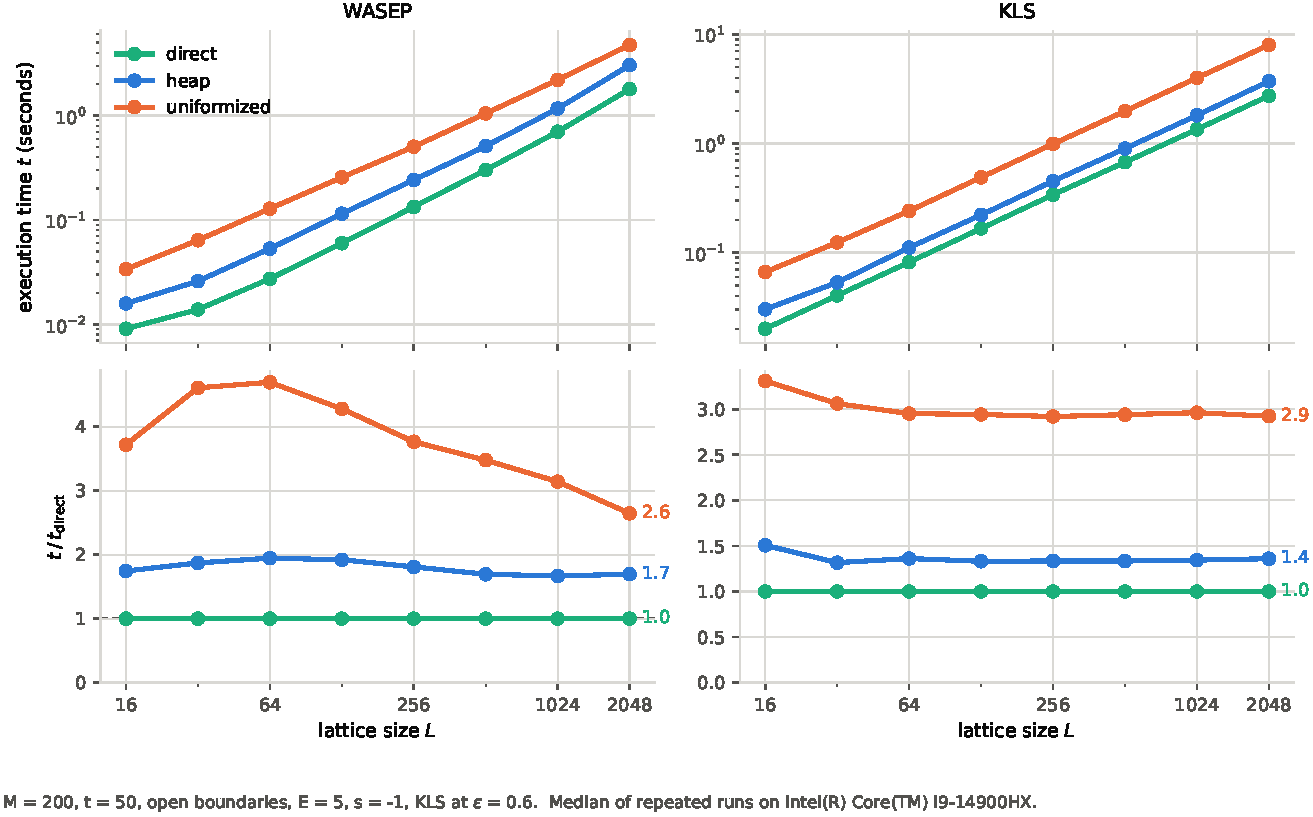
\includegraphics[width=\textwidth]{../../figures/scalability/scaling_length_mechanisms.pdf}
\caption{The three mechanisms against lattice size, at fixed population. Above,
the execution time of one run; below, the same divided by
\textcolor{dircol}{\textbf{Direct}} at the same size. Flat lower curves mean a
per-event cost that does not grow with $L$.}
\label{fig:scaling-length}
\end{figure}

\begin{figure}[tbp]
\centering
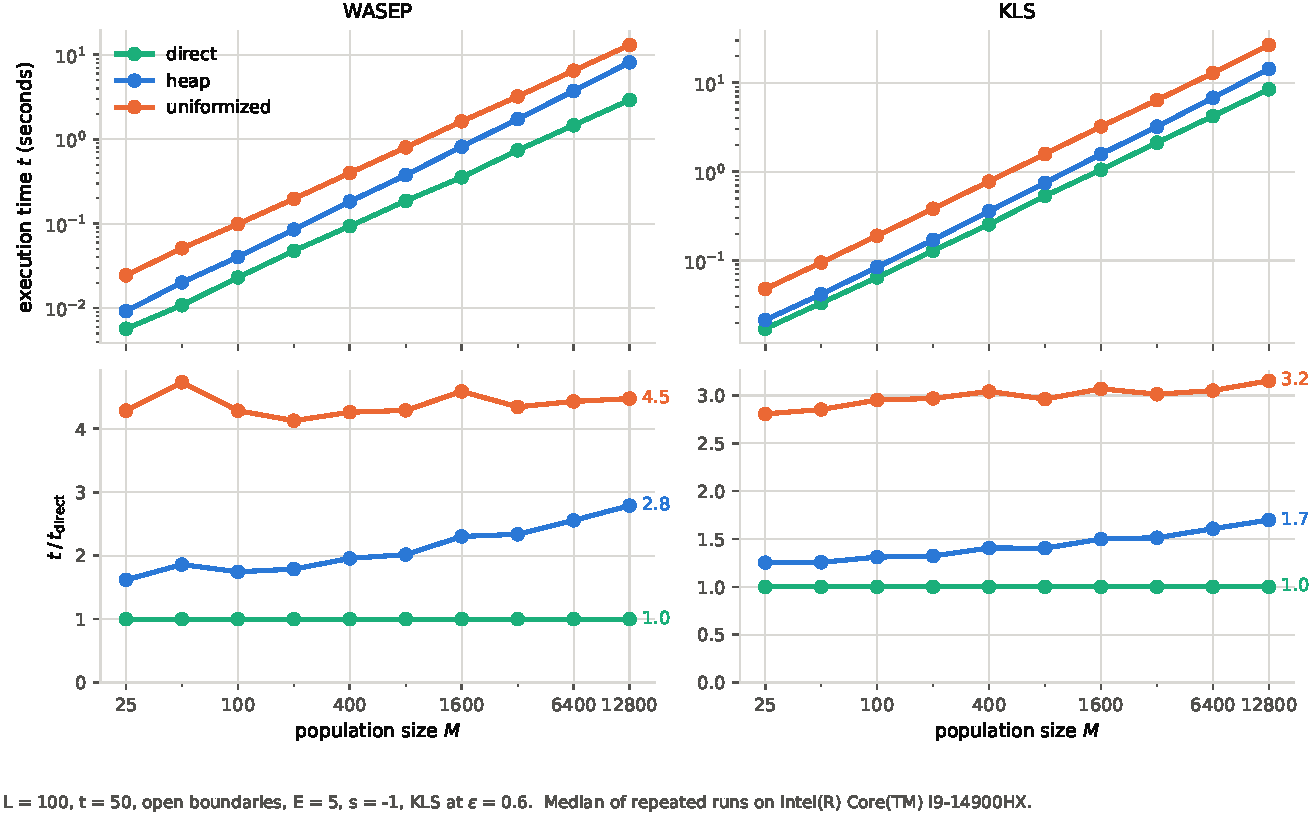
\includegraphics[width=\textwidth]{../../figures/scalability/scaling_walkers_mechanisms.pdf}
\caption{The same against population size, at fixed lattice. The rise of the
\textcolor{heapcol}{\textbf{Heap}} curve below is its $O(\log M)$ sift; the
\textcolor{unifcol}{\textbf{Uniformized}} one is flat, its rejections being a
per-event cost.}
\label{fig:scaling-walkers}
\end{figure}

The engine is checked against two kinds of tests. In the first, the tilted generator is written out in full and diagonalised for a small open chain, with its dominant eigenvalue being the cumulant generating function exactly. The diagonalisation in
\texttt{validation/exact/SSEP\_TM.py} spreads the counting field over the bonds exactly as the engine does, so the two report the same observable and their numbers compare directly. Below, $\alpha=\beta=1$ with $\gamma=\delta=0$, holding
the reservoirs at $\rho_{\rm L}=1$ and $\rho_{\rm R}=0$; the simulations use
$M=4000$ and $t_{\max}=4000$. No deviation exceeds $10^{-4}$. That is the statistical error of the estimate and not a disagreement between the mechanisms. 

\begin{center}
\begin{tabular}{ccc@{\hspace{1.5em}}ccc}
\hline
$L$ & $s$ & exact & \textcolor{dircol}{direct} & \textcolor{heapcol}{heap}
& \textcolor{unifcol}{uniformized} \\
\hline
5 & $-1$ & $-0.137095$ & $-0.137048$ & $-0.137058$ & $-0.137000$ \\
5 & $+1$ & $ 0.201977$ & $ 0.201963$ & $ 0.201945$ & $ 0.201933$ \\
6 & $-1$ & $-0.117955$ & $-0.117939$ & $-0.117980$ & $-0.117915$ \\
6 & $+1$ & $ 0.172403$ & $ 0.172360$ & $ 0.172368$ & $ 0.172381$ \\
8 & $-1$ & $-0.092207$ & $-0.092177$ & $-0.092170$ & $-0.092181$ \\
8 & $+1$ & $ 0.133351$ & $ 0.133319$ & $ 0.133341$ & $ 0.133367$ \\
\hline
\end{tabular}
\end{center}


In the second test we benchmark the engine against the analytical results found in~\cite{bodineau2004current}. With no external field and the reservoirs holding equal densities, the open SSEP has a cumulant generating function known in closed form, but only to leading order in $L$. Plotting the rescaled CGF $(L-1)\lambda(s)$ for different values of $L$, we observe in figure~\ref{fig:ssep-convergence} that the whole curve collapses onto the $L \to \infty$ analytical solution as the lattice grows. At fixed $s$ the approach is monotonic from
below.

\begin{figure}[tbp]
\centering
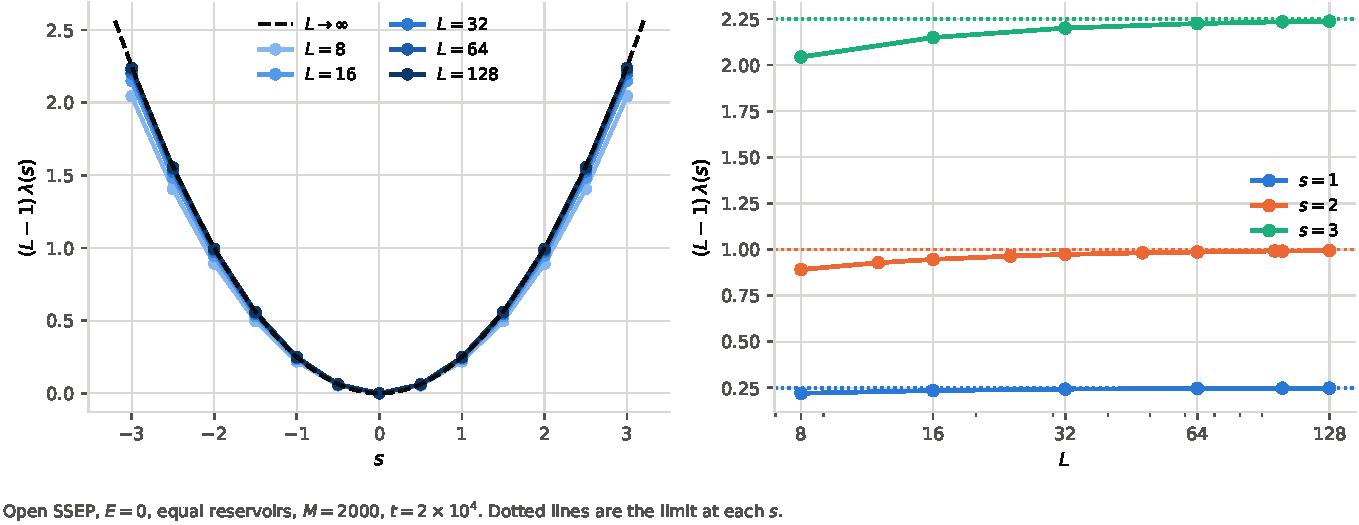
\includegraphics[width=\textwidth]{../../validation/figures/ssep_large_L_convergence.pdf}
\caption{The open SSEP against its large-$L$ closed form. Left, the rescaled
generating function over the whole counting field at several sizes; right, three
of those fields followed as the lattice grows, each limit dotted.}
\label{fig:ssep-convergence}
\end{figure}

\subsection{Parameter reference}
\label{sec:parameters}

Table containing every quantity the engine takes, spelled as it is written in the plan file (".toml"). 

\begin{center}
\begin{tabular}{llp{7.4cm}}
\hline
symbol & name in the plan & meaning \\
\hline
\multicolumn{3}{l}{\emph{Model and fields}} \\
$L$ & \texttt{length} & number of sites \\
--- & \texttt{model} & \texttt{WASEP}, \texttt{KLS} or \texttt{NNN}; selects
    where the eight rate-group weights come from \\
$\epsilon$ & \texttt{epsilon} & KLS coupling to the difference of the flanking
    occupations; $0$ recovers WASEP \\
$\delta_{\text{KLS}}$ & \texttt{delta\_kls} & KLS coupling to their sum; $0$
    preserves particle--hole symmetry.  \\
$w_\rightarrow, w_\leftarrow$ & \texttt{right\_weights},
    \texttt{left\_weights} & the four class rates per direction, given
    explicitly for \texttt{model = "NNN"} \\
$E$ & \texttt{field} & external driving field \\
$s$ & \texttt{bias} & counting field  \\
$k$ & \texttt{measurement\_strength} & monitoring coupling to the reference;
    $k = 0$ switches the reference off \\
\hline
\multicolumn{3}{l}{\emph{Boundaries}} \\
--- & \texttt{boundary} & \texttt{"open"} or \texttt{"periodic"} \\
$\rho$ & \texttt{filling} & periodic case: initial density \\
$\alpha, \gamma$ & \texttt{alpha}, \texttt{gamma} & open case:
    injection into, and removal from, the leftmost site \\
$\delta, \beta$ & \texttt{delta}, \texttt{beta} & open case: injection into,
    and removal from, the rightmost site \\
\hline
\multicolumn{3}{l}{\emph{Population and estimator}} \\
$M$ & \texttt{walkers} & population size \\
--- & \texttt{target\_min} & weight ratio at which resampling becomes
    worthwhile \\
--- & \texttt{target\_max} & weight ratio that must never be exceeded \\
--- & \texttt{cloning\_interval} & optional extra resampling on a fixed clock \\
\hline
\multicolumn{3}{l}{\emph{Run}} \\
$t_{\max}$ & \texttt{time} & final time \\
--- & \texttt{dynamics} & \texttt{"direct"}, \texttt{"heap"} or
    \texttt{"uniformized"}; the event mechanism, described in the
    mechanism note of Section~\ref{sec:algorithm} \\
--- & \texttt{initial} & initial configuration: \texttt{"empty"},
    \texttt{"alternating"}, \texttt{"random"} or \texttt{"full"}. Open chains
    only; a ring takes its particle number from \texttt{filling} \\
--- & \texttt{seed} & random seed; sweeping it gives independent repetitions \\
--- & \texttt{record\_interval} & time between recorded rows \\
\hline
\end{tabular}
\end{center}

\bibliographystyle{unsrt}
\bibliography{algorithm_refs}
\end{document}
